\chapter{Fundamentals and Related Work\label{cha:relatedwork}}

This chapter is intended to give an introduction about relevant terms, technologies and
standards in the field of Deep Learning and Generative Adversarial Networks. It also
covers some necessary backgrounds to get the basic overview of the topic.

\section{Classification using Deep Learning}
As we already mentioned in Chapter \ref{cha:introduction}, \acrfull{dl} is a powerful
\acrshort{ml} tool. It has a lot of advantages comparing to the other traditional methods.
In many cases, it does not need a thorough and careful Feature Extraction, and the
multiple-layer nature enable it to learn multiple levels of features from the data. In
this section, the author would like to discuss some relevant backgrounds on \acrshort{dl}
and how people use it for Object Classification.

Classification is a basic task in \acrshort{ml}, and Image Classification has become a
very common application of Deep Learning since the beginning because of the potential
applications, availability of data, and the pixel structure of the images in which every
pixel can be assumed to be independent from the other. The last point is a very important
assumption in a lot of \acrshort{ml} applications. 

Because of the popularity of the topic, a lot of researchers have been spending efforts on
designing and training different architectures to get the best results.  Different works
are usually evaluated on some standard labeled datasets. The accuracies on those datasets
are considered as the performance metric of a network. ImageNet \cite{imagenet} is
one of the biggest and most popular Object Image Database available, consisting of
millions of images. On ImageNet, Krizhevsky et al. \cite{alexnet} trained an 8-layer
Convolutional Neural Networks which achieved significantly lower error rates than the
State-Of-The-Art methods at the publication time.

\subsection{Transfer Learning}
If we take a closer look at a Deep Classification Network such as AlexNet \cite{alexnet}, we can see that the last layer is often a Softmax layer, which does nothing more
than converting the output to the range $[0, 1]$ so that we have a prediction probability
of each class. The real classification work is done in the previous layer (fc8), where the
probability that the object image belongs to each class is calculated by a Linear
Regression. In AlexNet, as we have 1000 classes, we have 1000 neurons in fc8 corresponding
to 1000 Linear Regressions. The intuition here is that, the input of that decision layer
should be a good representation of the data if the network is performing well. In
principle, we can reuse the output of the layer before fc8, which is fc7, in other
\acrshort{ml} tasks. That forms the basic idea of Transfer Learning.

\subsection{AlexNet}
As mentioned above, AlexNet is one of the classical approaches of using Deep Neural
Network to solve the Object Classification task on the huge dataset ImageNet.  AlexNet
consists of 8 layers as shown in Figure~\ref{fig:alexnet}. There are 5 convolutional
layers and 3 fully-connected layers. The last layer is connected to a 1000-way Softmax
layer because the ImageNet dataset \cite{imagenet} used to train the network contains
1000 classes.

\begin{figure}[htb]
  \centering
  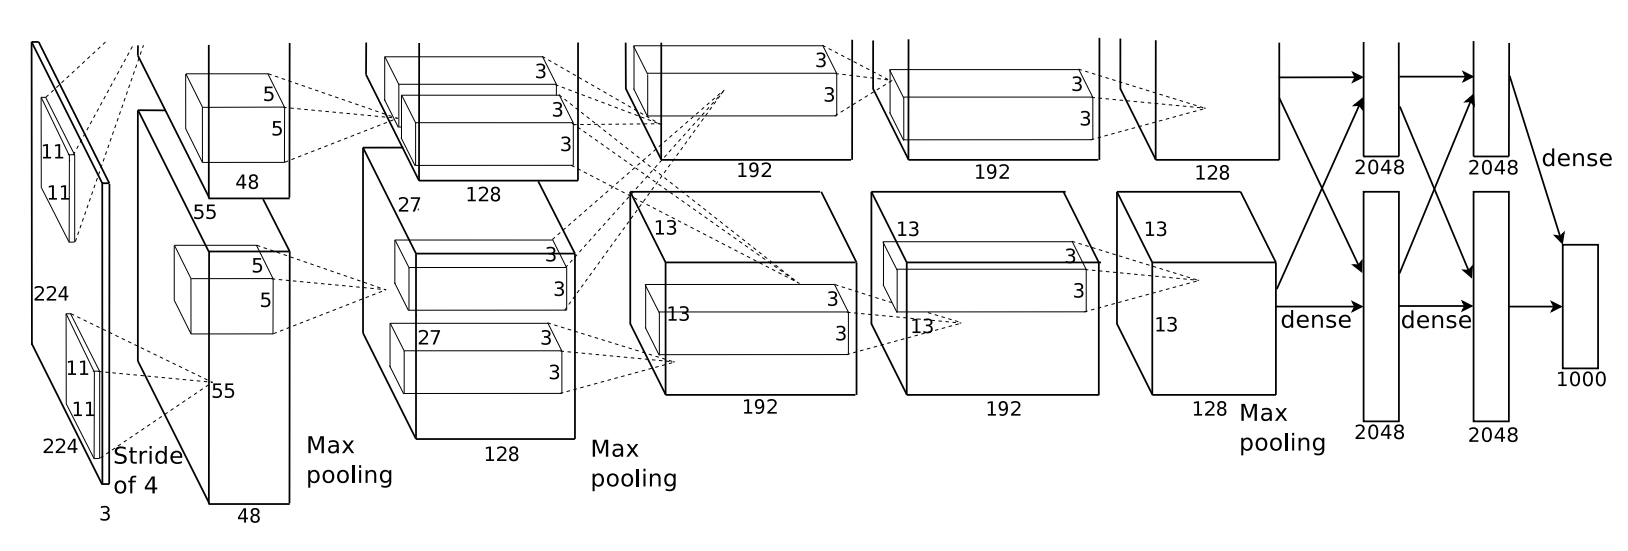
\includegraphics[width=0.9\textwidth]{alexnet_architecture}
  \caption{AlexNet Architecture}\label{fig:alexnet}
\end{figure}

\subsection{Object Recognition on Washington RGB-D dataset \cite{eitel}}
Transfer Learning is the main idea of Eitel et al. \cite{eitel}. In the paper, the
authors use an implementation of AlexNet in Caffe (CaffeNet) to get the representations of
the objects in the Washington RGB-D dataset. The representations are then fed into a
fully-connected layers, where the final results are connected to a 51-way Softmax layers, to
classify 51 different classes in the Washington Object Dataset \cite{washington_rgbd}.
Figure \ref{fig:eitel_net} describes the network.

\begin{figure}[htb]
  \centering
  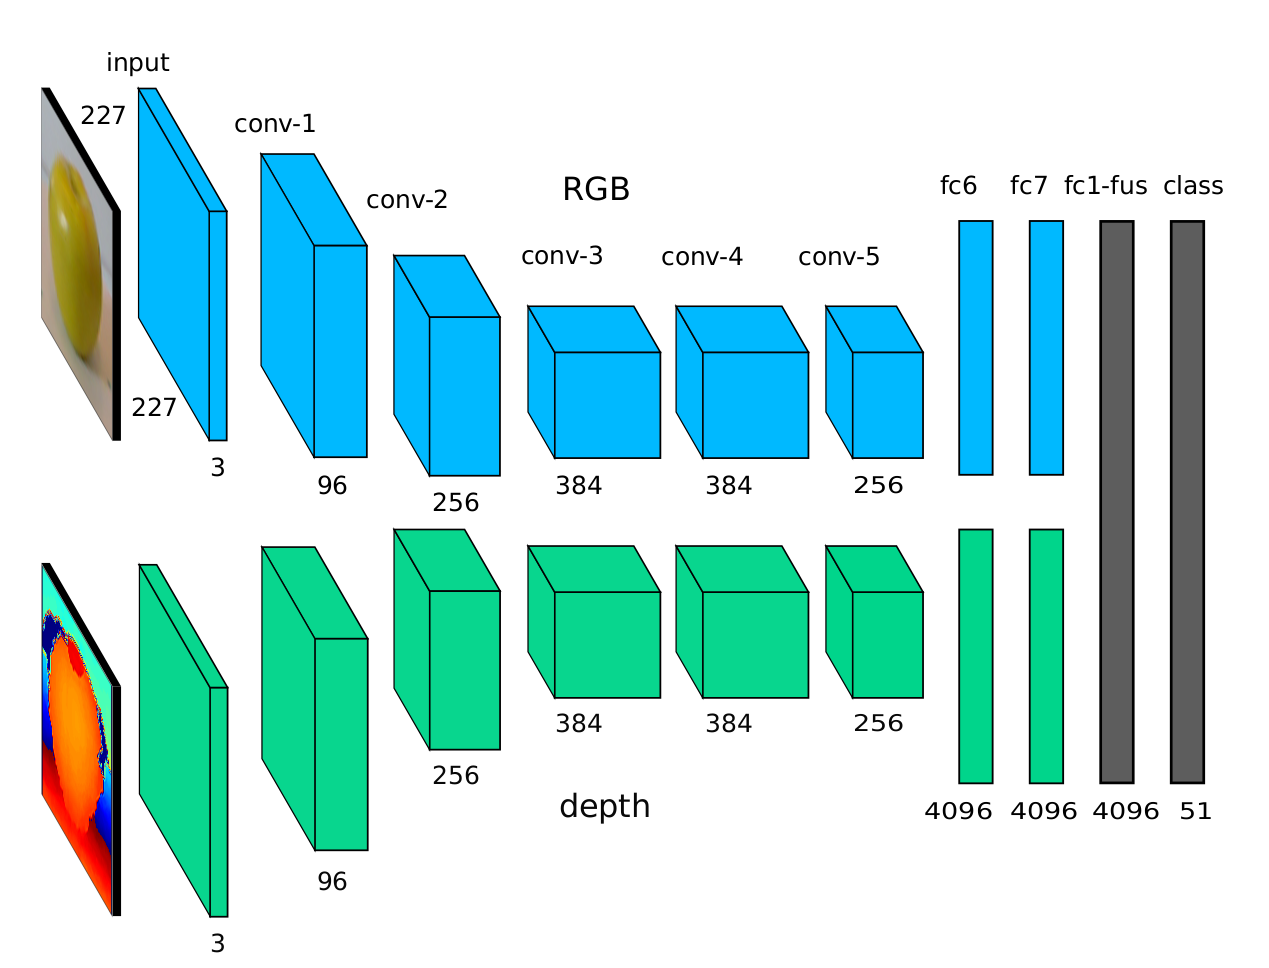
\includegraphics[width=0.9\textwidth]{eitel_net}
  \caption{Eitel et al. architecture for Object Classification}\label{fig:eitel_net}
\end{figure}

\section{\acrfull{gan}}
In 2014, {\acrlong{gan}} was proposed by Ian Goodfellow \cite{gan}. It immediately
created a new trend as a very hot topic in the Deep Learning community. \acrshort{gan}
consists of two differentiable functions, usually in forms of Deep Neural Networks. One is
basically a Generative Model which tries to learn a distribution from the training data
and to be able to draw new samples from that distribution. The other is a classifier whose
job is to tell whether a sample is from the original data or is generated by the first
component. Based on the roles, the former is called the Generator and the latter is called
the Discriminator.

There can be different design for the two networks depending on the domain that
\acrshort{gan} is applied. In Computer Vision applications, it is common that the
Generator is a Deep Convolutional Neural Network which behaves in a similar way as an Auto
Encoder \cite{auto_encoder} works. The first half is an Encoder where an image is
reduced to a representation of 1D array, then the second half tries to decode that
representation to the original image. In this case, the difference is that this Generator
does not minimize the direct loss between the output and the input. Instead, it tries to
maximize the loss of the Discriminator. The Discriminator, in another way, is a binary
classifier who tries to distinguish the original image and the output image from the
Generator. 

In the most basic setting, the Discriminator always receives a pair of inputs:

\begin{itemize}
	\item Target: The ground-truth from the dataset, also called "Real Item". Label 1
	\item Output: The product of the Generator, also called "Fake Item". Label 0
\end{itemize}

Let $G$ denotes the generating function and $D$ denotes the classification function and
given an arbitrary image $x$, then $G(x)$ is also an image and $D(x)$ is a scalar label where
$D(x) \in {0, 1}$.

Obviously, the goal of the Discriminator is to assign label 1 for all the real
images and label 0 for all the fake images. Thus the Discriminator Loss is
a Cross-Entropy between the output of the Discriminator and the set of labels ${0, 1}$. In
other words, the Discriminator maximizes the probability of assigning the correct labels
to its inputs by maximizing the Value Function $V(D) = \log(D(x)) + \log(1 - D(G(z)))$.

At the same time, the goal of the Generator is to "create troubles" for the
Discriminator. Particularly, it tries to make the Discriminator think that its output is
"real" (label 1), meaning it minimizes the second component of the Discriminator Value
Function $\log(1 - D(G(z)))$.

Based on the setting above, we end up in a two-player minimax game with the 
following value function:

\begin{align*}
	\min_{G} \max_{D} V(D, G) = \mathbb{E}_{x \sim p_{data}(x)} [\log D(x)] +
	\mathbb{E}_{z \sim p_z(z)}[\log(1 - D(G(z)))]
\end{align*}

In practice, for implementation purpose, people usually set the Discriminator Loss to be
$L(D) = -V(D, G)$ so that we can use Gradient Descent to minimize it and utilize the
existing Deep Learning frameworks. The Generator is also set to maximize $\log(D(G(z)))$,
equivalent to minimizing $-\log(D(G(z)))$, instead of minimizing $\log(1 - D(G(z)))$
because the latter has problems of vanishing gradients, shown in \cite{gan}.

We can see that the Discriminator job is as simple as any other binary classifier, it
distinguishes the real data distribution $p_{data}$ from the Generator outcome
distribution $p_{g}$. In order to "fool" it, the Generator has to learn the data
distribution $p_{data}$. In every step, the optimal Discriminator is $D^{*}(x) =
\frac{p_{data}(x)}{p_{data}(x) + p_{g}(x)}$, the proof is provided in \cite{gan}. When the system reaches an equilibrium, $p_{g}$ should converge to $p_{data}$,
thus the optimal Discriminator Outcome should be $D^*(x) = 0.5$, equivalent to a Value
Function $\log(0.5) + \log(0.5) = -1.38629436112$.

As an example, if we want to learn a cat image distribution, the Generator will draw
synthesized cat images from an arbitrary input $z$, and the Discriminator will try to tell
that the output cat image is a "fake" one and an arbitrary image from the data is a "real"
one. When the two networks converge, we should have an implicit model representing a cat
image distribution.

\section{Conditional \acrshort{gan} and Pix2pix}
The original non-conditional \acrshort{gan} is sometimes referred as the "Vanilla
\acrshort{gan}". It sets up good foundation for the field, but is sometimes unstable and
hard to train. In some applications, people are not interested in the general distribution
but rather pay attention to a directed data generation, that is, a conditional
distribution. For instance, generating a random cat may not be as interesting to somebody
as creating an image of a Bengal cat. Just shortly after the introduction of
\acrshort{gan}, Mirza and Osindero \cite{cogan} proposed Conditional GANs, an improved
version of \acrshort{gan}. The idea is simple, instead of generate from an arbitrary noise
input $z$, the Generator also takes another vector $y$ as the condition. In the example of
cat image generation, we can provide a Bengal cat image, a string "Bengal", or a binary
label vector as $y$. The Discriminator also takes $y$ as its condition. By being trained
in that way, \acrshort{gan} now learns a conditional model $p_{g}(x|y)$ and tries to make
it as close as the conditional distribution of the data $p_{data}(x|y)$ as much as
possible. Figure \ref{fig:co_gan_model} demonstrates how conditional \acrshort{gan} works.

\begin{figure}[h]
	\centering
	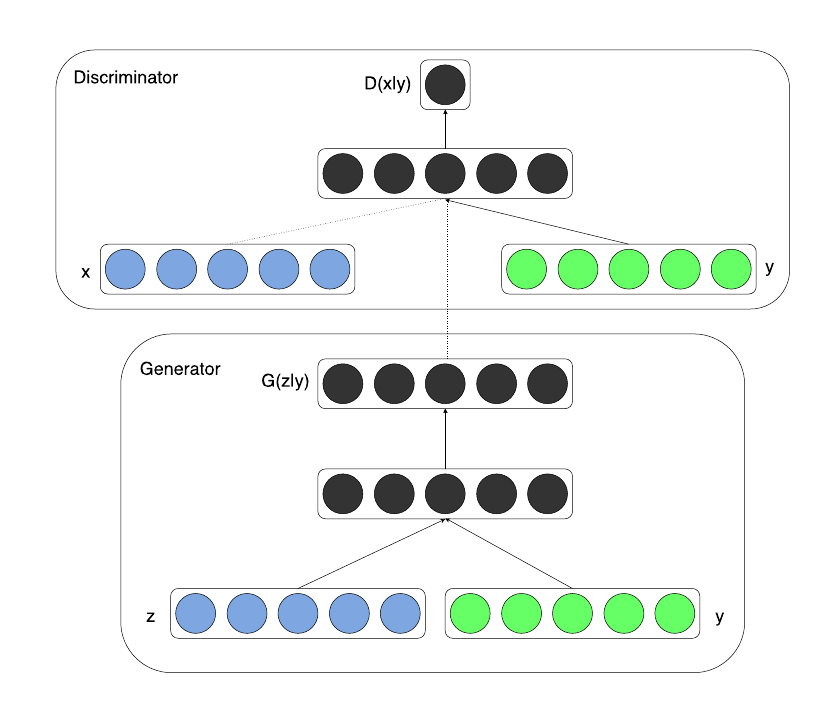
\includegraphics[width=0.5\linewidth]{img/co_gan_model}
	\caption{Conditional \acrshort{gan}s}
	\label{fig:co_gan_model}
\end{figure}

\begin{figure}[h]
	\centering
	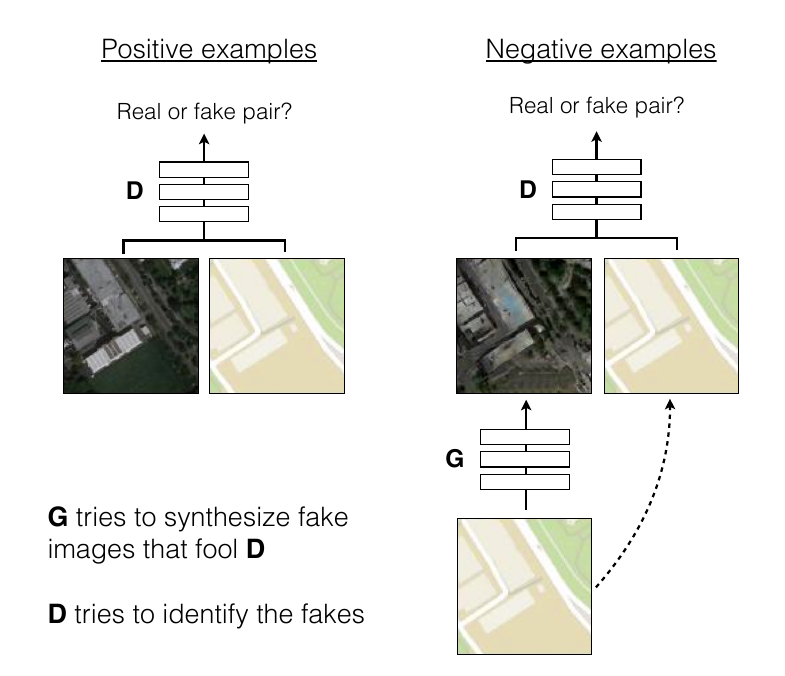
\includegraphics[width=0.5\linewidth]{img/pix2pix_workflow}
	\caption{How \acrshort{pix} works.}
	\label{fig:pix2pix_workflow}
\end{figure}

Conditional GANs have many applications, \acrfull{pix} \cite{pix2pix} is an example.
It maps an image to another image. The authors demonstrate that \acrshort{pix} is able to
generate satellite images from map views and vice versa, detailed buildings with texture
from skeleton sketches, or day to night transformation. Those impressive results come from
the idea of conditioning a \acrshort{gan} on an input image. In figure
\ref{fig:pix2pix_examples}, we can see some outputs of \acrshort{pix} from the authors.
The general workflow is demonstrated in Figure~\ref{fig:pix2pix_workflow}.

\begin{figure}[h]
	\centering
	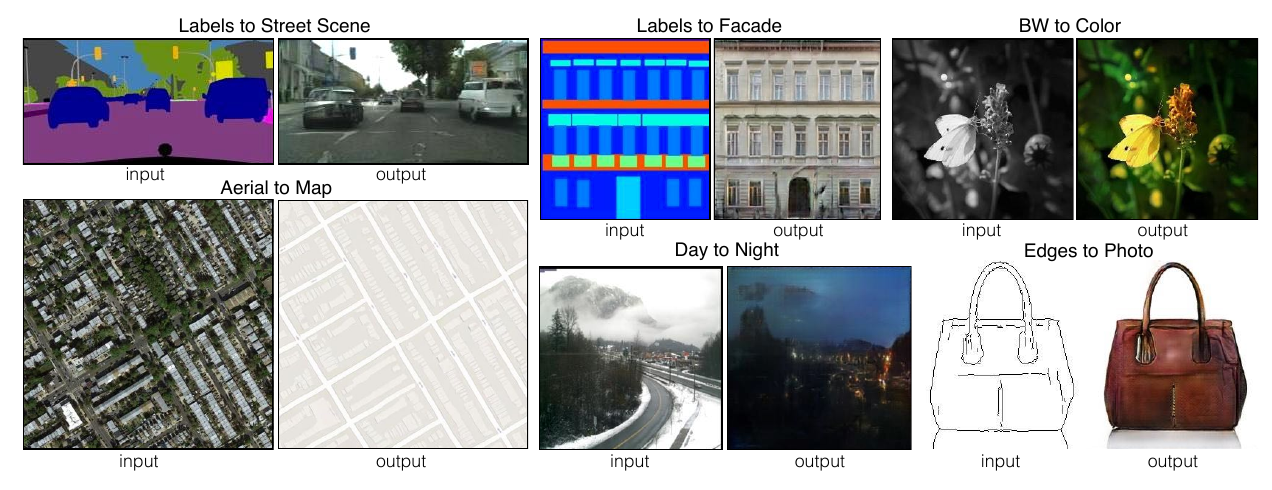
\includegraphics[width=0.8\linewidth]{img/pix2pix_examples}
	\caption{Examples of \acrshort{pix} from the authors}
	\label{fig:pix2pix_examples}
\end{figure}

As this is a conditional \acrshort{gan}, the loss function is also a little bit different
from the Vanilla \acrshort{gan} in the sense that all the components now are conditional
on an image $y$.  Besides, the authors also suggest using an L1 loss to boost up the
Generator training as it helps the Generator learns faster and L1 enforces less blurry
images than L2.

\begin{align*}
	\min_{G} \max_{D} V(D, G) = \mathbb{E}_{x \sim p_{data}(x)} [\log D(x, y)] +
	\mathbb{E}_{z \sim p_z(z)}[\log(1 - D(G(y, z), y))] \\ 
	+ \lambda L1(G)
\end{align*}
